\documentclass[11pt]{article}
\usepackage{amsmath,textcomp,amssymb,geometry,graphicx,enumerate,tikz}

\def\Name{Vijay Hans}  % Your name
\def\SID{3041285081}  % Your student ID number
\def\Prelab{5} % Number of Prelab
\def\Session{Spring 2026}
\def\Cls{PHYS 5BL}
\title{\Cls--Spring 2026 --- Prelab \Prelab \ Response}
\author{\Name, SID \SID}
\markboth{\Cls -- \Session\  Prelab \Prelab \ \Name}{\Cls -- \Session\ Prelab \Prelab\ \Name}
\pagestyle{myheadings}
\date{\today}

\newenvironment{qparts}{\begin{enumerate}[{(}a{)}]}{\end{enumerate}}
\def\endproofmark{$\Box$}
\newenvironment{proof}{\par{\bf Proof}:}{\endproofmark\smallskip}

\textheight=9in
\textwidth=6.5in
\topmargin=-.75in
\oddsidemargin=0.25in
\evensidemargin=0.25in
\setlength{\parindent}{0pt}
\begin{document}
\maketitle

\begin{enumerate}
    \item \begin{enumerate}
              \item Assuming the split is in the middle of the rod, the situation is symmetric about the rod's midpoint, so the expected length is $\frac{L}{2}$.
              \item Let $x$ and $y$ be the lengths of the rod at hand. We then have the condition $x+y = L$ and we hope to find $E[\min(x,y)]$. In the picture below, we draw these conditions, along with the line $x=y$.\\
                    \begin{center}
                        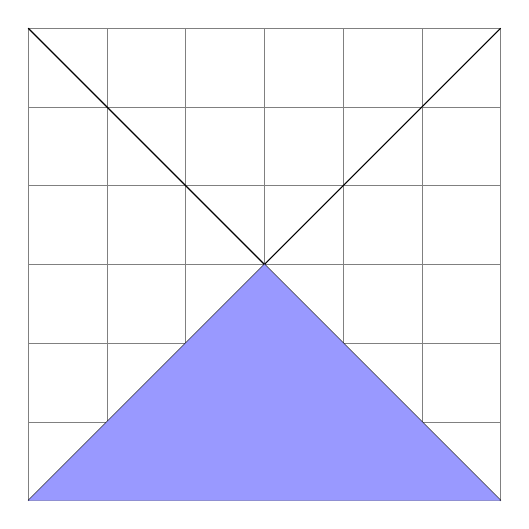
\begin{tikzpicture}
                            \draw[step=1cm,gray,very thin] (0,0) grid (6,6);
                            \draw (6,0) -- (0,6);
                            \draw (0,0) -- (6,6);
                            \fill[blue!40!white] (0,0) -- (3,3) -- (6,0) -- cycle;
                        \end{tikzpicture}
                    \end{center}
          \end{enumerate}
          The shaded triangle in the diagram describes the minimum desired, so we hope to find its average height. This is the quotient of the area and the length of the base, or half the altitude, giving $\frac{L}{4}$.
\end{enumerate}

\end{document}